\documentclass[paper=a4, fontsize=11pt]{scrartcl}
\usepackage[T1]{fontenc}
\usepackage{fourier}

\usepackage[english]{babel}															% English language/hyphenation
\usepackage[protrusion=true,expansion=true]{microtype}	
\usepackage{amsmath,amsfonts,amsthm} % Math packages
\usepackage[pdftex]{graphicx}	
\usepackage{url}
\usepackage{hyperref}

%%% Custom sectioning
\usepackage{sectsty}
\allsectionsfont{\centering \normalfont\scshape}
\usepackage{subfigure}

\usepackage{comment}


%%% Custom headers/footers (fancyhdr package)
\usepackage{fancyhdr}
\pagestyle{fancyplain}
\fancyhead{}											% No page header
\fancyfoot[L]{}											% Empty 
\fancyfoot[C]{}											% Empty
\fancyfoot[R]{\thepage}									% Pagenumbering
\renewcommand{\headrulewidth}{0pt}			% Remove header underlines
\renewcommand{\footrulewidth}{0pt}				% Remove footer underlines
\setlength{\headheight}{13.6pt}


%%% Equation and float numbering
%\numberwithin{equation}{section}		% Equationnumbering: section.eq#
%\numberwithin{figure}{section}			% Figurenumbering: section.fig#
%\numberwithin{table}{section}				% Tablenumbering: section.tab#


%%% Maketitle metadata
\newcommand{\horrule}[1]{\rule{\linewidth}{#1}} 	% Horizontal rule

\title{
		%\vspace{-1in} 	
		\usefont{OT1}{bch}{b}{n}
		%\normalfont \normalsize \textsc{CS650 - Computer Vision} \\ [25pt]
		%\horrule{0.5pt} \\[0.4cm]
		%\huge Programming Lab 2 \\ Edge Detection / Hough Transform \\
		Multi-objective path planning
		\horrule{2pt} \\[0.5cm]
}
\author{
		%\normalfont 								\normalsize
        Daqing Yi\\[-3pt]		\normalsize
        \today
}
\date{}


%%% Begin document
\begin{document}
\maketitle

\section{Introduction}

\begin{frame}{Modeling human intent}{Path Planning}
THe problem in modeling human intent
\begin{itemize}
\item incomparability in objectives
\item conflict in objectives
\item hardness in weighing the objectives
\item vagueness in importance selection
\end{itemize}
\begin{figure}
\centering
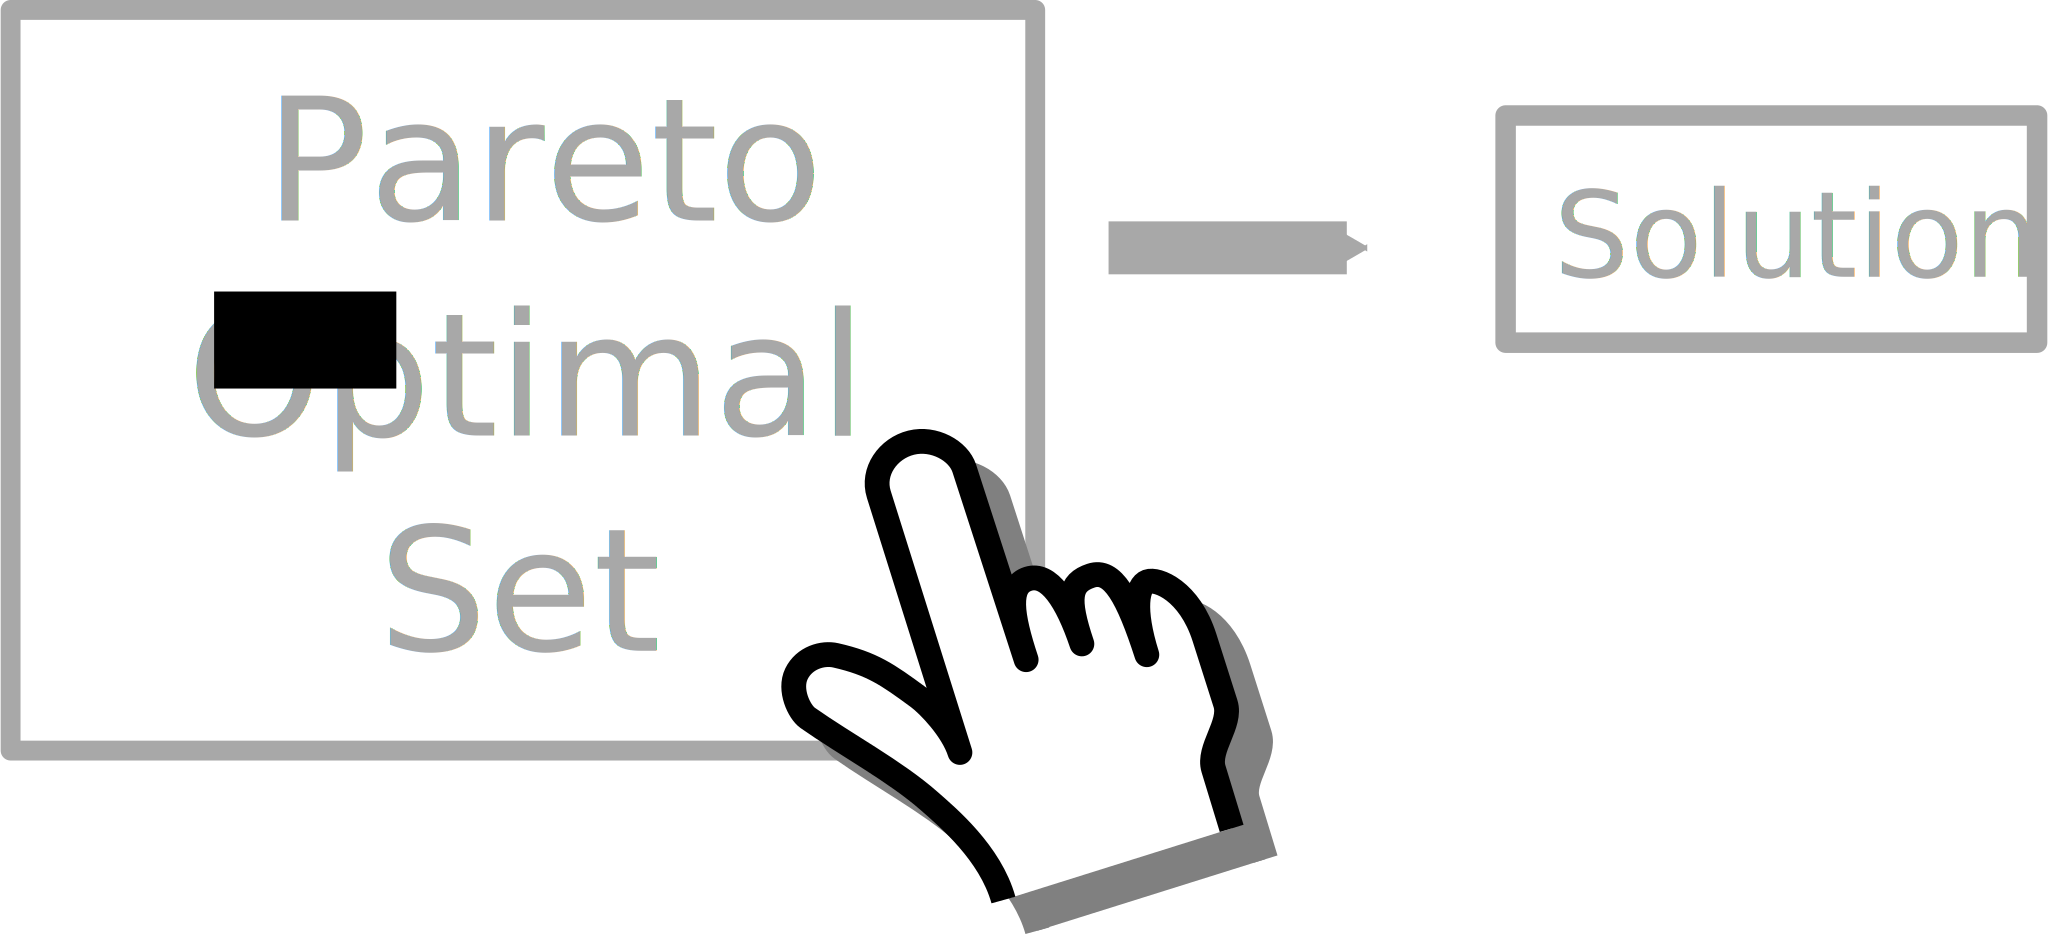
\includegraphics[width=0.6\linewidth]{figure/human_interactive_moo}
%\caption{}
\label{fig:human_interactive_moo}
\end{figure}
\end{frame}

\begin{frame}{Pareto Optimal}{}
\end{frame}

\section{Homotopy}

In a map without obstacles, the solution space is compact.
The import of obstacles breaks the compactness.
However, when there are a start point and an end point, a homotopy class of trajectories can be defined in a map with obstacles.
A \textbf{homotopy class} of trajectories is defined by the set of trajectories joining same start and end points which can be smoothly deformed into one another without intersecting obstacles~\cite{bhattacharya2010search}.




\bibliographystyle{plain}
\bibliography{reference}

\end{document}